% chapter2.tex (Chapter 2 of the thesis)

\chapter{Assessment of Harmonic Based Techniques and Repertoire}

% TODO: Talk about Pythagoreas.
Harmonic based techniques invariably make use of the harmonic series in one way or another. The harmonic series is a sequence of tones in which the frequency of each is an integer multiple of the fundamental frequency. The earliest forms of tuning systems were based around these, but modern instruments are tuned around equal temperament.

\subsection{Background}
Provide an overlay of the techniques and explain how they work, the general benefits and such.
\subsection{Research statement/problem}
Techniques are under-developed and/or under-used.

\subsection{Aim and scope of thesis}
Examples of use in current literature will support use-case scenarios, dearths of usage will support the fact that they are underused.

\subsection{Significance of work}
The production of technique and its uses.

\section{Subharmonics}
% TODO: Explain subharmonics
First discovered by Mari Kimura, subharmonics are a type of overpressure which produces a sound lower than the fundamental.\autocite{kimuraHowProduceSubharmonics1999}  When the bow is drawn across the string, the drag of the bow twists the string, creating torsional oscillation. Under the right conditions, these can interact with the string to produce an identifiable pitch lower than the fundamental.\autocite{Subharmonics2006} \lipsum[3]


\subsection{Works featuring subharmonics}
One of the newest string techniques, subharmonics are still in their comparative infancy, and their notation has not been formalised. There have been several different ways of notating them, each with their advantages and disadvantages.
% TODO: Find pieces using subharmonics


\begin{figure}
    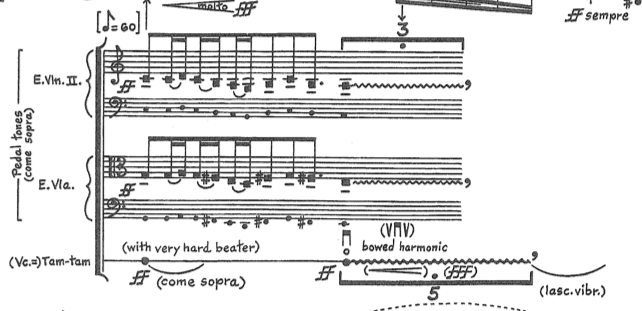
\includegraphics[width=\linewidth]{./resources/crumbBlackAngels.png}
    \caption{Excerpt from Crumb's Black Angels.}
    \label{fig:Excerpt from Crumb's Black Angels}
  \end{figure}
% TODO: Citation needed for Crumb
Possibly the first person to make use of the technique, Crumb described subharmonics as `pedal tones'. The use of square noteheads and a separate stave for the resultant pitch makes the technique clear and readily understandable.
% TODO: Citation needed for `pedal tones'

\begin{figure}
    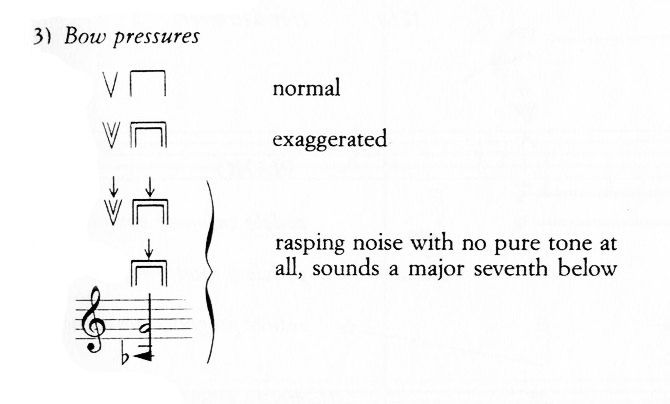
\includegraphics[width=\linewidth]{./resources/griseyVortexTemporum.jpg}
    \caption{Excerpt from Grisey's playing instructions for Vortex Temporum.}
    \label{fig:Excerpt from Grisey's playing instructions for Vortex Temporum}
  \end{figure}
% TODO: Citation needed for Grisey
Gerard Grisey's \emph{Vortex Temporum} features overpressure, with a subharmonic of specifically a seventh. Somewhat abstracted out, this hides the intended effect behind symbols, and is slower to sight read.

\begin{figure}
    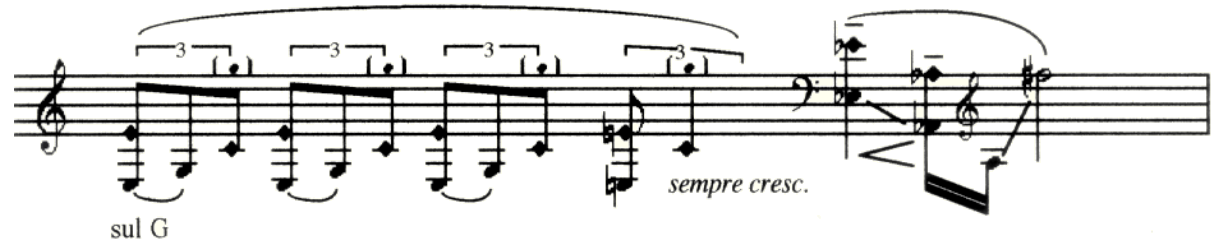
\includegraphics[width=\linewidth]{./resources/kimura_gemini.png}
    \caption{Excerpt from Kimura's Gemini.}
    \label{fig:Excerpt from Kimura's Gemini}
  \end{figure}
  % TODO: Citation needed for Gemini
  Mari Kimura's `Gemini' is an example of idiomatic usage of subharmonics on the violin. Kimura's notation practice of using a harmonic denoting the intended pitch below the fundamental is similar to the standard notation of harmonics, which Gould states is to `write harmonics as the player will finger them.'\autocite[413]{gouldBars2011} Unfortunately, this method proved somewhat counterintuitive in practice, as the notation was too similar, and caused sight reading issues.

Notationally, the best practice appears to be following Crumb's approach, condensing into one stave where possible. Musicians are better at sight reading above the stave than below the stave, so unlike natural harmonics, the need to split into another stave to show the resultant pitch is likely to be more common for composers wishing to use subharmonics. Below, I demonstrate the use of subharmonics twice in my work \emph{The Veldt}, for solo viola.
% TODO: Add figure for The Veldt

\section{Multiphonics}
% TODO: Explain multiphonics
Multiphonics on stringed instruments are difficult, but with appropriate preparation and notation, are quite feasible. Production of multiphonics, as with wind instruments, is not guaranteed, and can be dependant on a variety of external factors, including the humidity, make of the instrument, bow used, and other variables that are outside of the control of a composer.

% TODO: Expand Fallowfield discussion.
Fallowfield explores multiphonic production on the cello in her thesis CelloMap.\autocite{fallowfieldCelloMapHandbook2009} \lipsum[2]

\subsection{Works featuring multiphonics}
% TODO: Find multiphonic works
\lipsum[4]

\section{Electronically-Assisted Harmonics}
% TODO: Expand electronic assisted harmonics.
The use of electronics to augment acoustic instruments is hardly a new technique, although their use in a live context is still relatively inaccessible. For my composition `The Veldt', I will be making use of Max MSP, a patch-based audiovisual processing application. 

\subsection{Works featuring electronically assisted harmonics}
% TODO: Find works featuring electronically assisted harmonics
\lipsum[4]
